\chapter{Feature Extraction}
\label{ch:FeatureExtraction}

Before diving into the novelty detection framework itself, the features to be used need to be defined and extracted from the data. Since our goal is to detect a novel behaviour, we are interested in both \quoted{time-domain} and \quoted{frequency-domain} features. The former are used to capture the temporal evolution of the signal, while the latter are used to capture the spectral content of the signal. 
In this chapter, we will first introduce the reference dataset that will be used to test the framework and then we will describe the features that will be used in the framework. The \gls{nd} framework will work on the complete collection of teatures $\vect{F}=\{\vect{F}_t, \vect{F}_f\}$, where $\vect{F}_t$ is the collection of time-domain features and $\vect{F}_f$ is the collection of frequency-domain features. Some of the featires will be extracted for all the signals available, while some other only on a subset of the signals, depending on the settings of the framework, as we will see in \autoref{ch:Framework}. 



\section{Reference dataset}
In the field of \gls{nd}, a famous bearing vibration dataset has been collected from the Center for Intelligent Maintenance Systems (\gls{ims}) of the University of Cincinnati and made available online on the \gls{nasa} website \cite{lee2007bearingdataset}. 
Let's take this as a starting point for our work. The dataset contains the vibration measurements collected at a sampling frequency $f_s=20\si{\kHz}$ of four forced-lubricated bearings. The shaft was kept constant at $2000$rpm during the data collection. The test rig is shown in \autoref{fig:IMS_bearing_dataset} and the test parameters are summarized in \autoref{tab:IMS_test_parameters}, that also shows the type of faults that happened in each repetiotion of the test.

To visualize what appens to the vibration signal as the bearing degrade over time, let's consider the \quoted{Bearing 3 x} signal from the \gls{ims} dataset, shown in \autoref{fig:IMS_bearing}. The top plot shows the vibration of the new bearing, while the bottom plot shows the vibration of the bearing just before the test was stopped. It's evident that the degraded signal reaches grater peaks in vibration and have a grater variance. The narrow peaks in the degraded signal are due to the presence of the fault frequencies, that are not present in the new bearing signal.

\begin{figure}
    \centering
    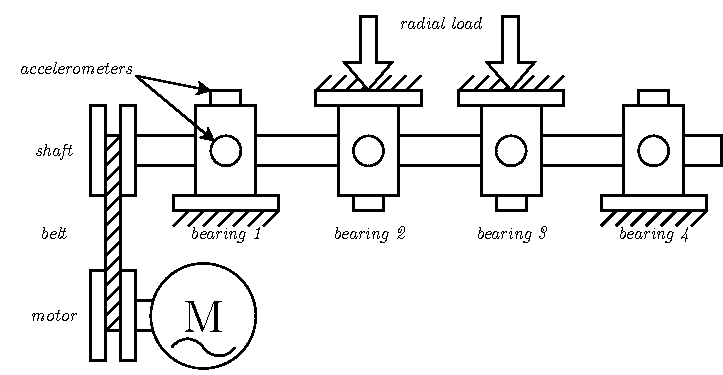
\includegraphics[scale=1]{images/FeatureExtraction/testrig.pdf}
    \caption{The test rig used by \cite{lee2007bearingdataset}}
    \label{fig:IMS_bearing_dataset}
\end{figure}

\begin{figure}
    \centering
    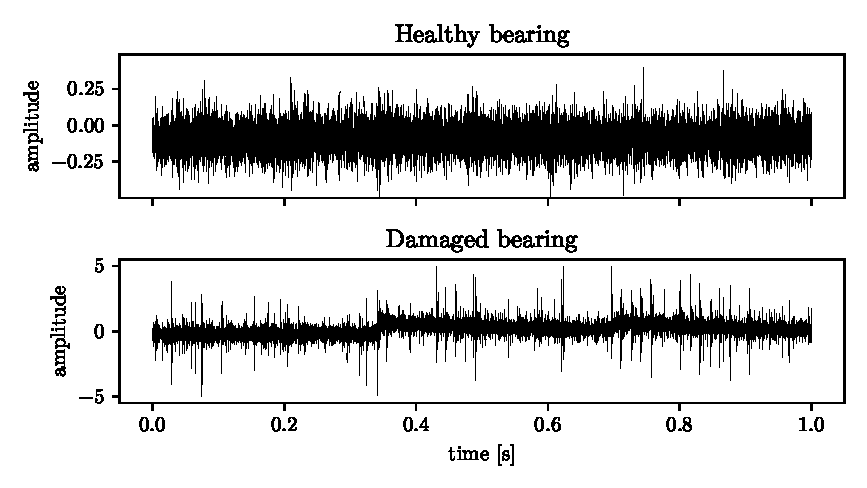
\includegraphics[scale=1]{images/FeatureExtraction/TD_signal.pdf}
    \caption{\quoted{Bearing 3 x} vibration signal from the \gls{ims} dataset}
    \label{fig:IMS_bearing}
\end{figure}

% \usepackage{tabularray}
\begin{table}
    \centering
    \caption{Test setup \cite{lee2007bearingdataset}}
    \label{tab:IMS_test_parameters}
    \resizebox{\linewidth}{!}{%
    \begin{tblr}{
      cell{2}{1} = {t},
      cell{2}{2} = {t},
      cell{3}{1} = {t},
      cell{3}{2} = {t},
      cell{5}{1} = {t},
      cell{5}{2} = {t},
      cell{6}{1} = {t},
      cell{6}{2} = {t},
      cell{7}{1} = {t},
      cell{7}{2} = {t},
      hline{1,8} = {-}{0.08em},
      hline{2} = {-}{},
    }
     & \textbf{Set No. 1} & \textbf{Set No. 2} & \textbf{Set No. 3}\\
    \textbf{Recording Duration} & 22/10/2003 - 25/11/2003 & 12/02/2004 - 19/02/2004 & 04/03/2004 - 04/04/2004\\
    \textbf{No. of Files} & 2156 & 984 & 4448\\
    \textbf{No. of Channels} & 8 & 4 & 4\\
    \textbf{Channel Arrangement} & {Bearing 1 ch 1  2\\Bearing 2 ch 3  4
    \\Bearing 3 ch 5  6
    \\Bearing 4 ch 7 \& 8~ ~~} & {Bearing 1 ch 1\\Bearing 2 ch 2\\Bearing 3 ch 3\\Bearing 4 ch 4 ~} & {Bearing 1 ch 1\\Bearing 2 ch 2\\Bearing 3 ch 3\\Bearing 4 ch 4~ ~~}\\
    \textbf{File Recording Interval} & 5 or 10 min & 10 min & 10 min\\
    \textbf{Fault type } & {Bearing 3: inner race defect\\Bearing 4: roller element defect} & Bearing 1: outer race failure & Bearing 3: outer race failure
    \end{tblr}
    }
    \end{table}

\section{Time-domain features}
Let's consider a timeserie $\vect{x}$ containing $n$ samples $x_1, x_2, \dots, x_n$. The goal of the feature extraction process is to extract a set of features $\vect{F}_t = \{F_1, F_2, \dots, F_m\}$ that can be used to describe the signal. In this section, we will describe the features that will be used in the developed framework.
\paragraph{Mean}
The first feature to be considered is simply the mean of the signal. It is defined as
\begin{equation}
    \mu = \frac{1}{n}\sum_{i=1}^n x_i
\end{equation}

\paragraph{\gls{rms}}
The Root mean square of the signal \gls{rms} is related with the power and is defined as
\begin{equation}
    \text{RMS} = \sqrt{\frac{1}{n}\sum_{i=1}^n x_i^2}
\end{equation}

\paragraph{Peack-to-peak}
The peak-to-peak value of the signal is defined as
\begin{equation}
    \text{P2P} = \max(\vect{x}) - \min(\vect{x})
\end{equation}

\paragraph{Standard deviation}
The standard deviation is a measure of the dispersion of the signal and is defined with respect a known distribution with knowledge of the true mean $\mu_{true}$ as

\begin{equation}
    {\sigma} = \sqrt{\frac{1}{n}\sum_{i=1}^n (x_i - \mu_{true})^2}
\end{equation}

but since in our case we don't know the true mean, we will use the sampled standard deviation, that is the best estimate, defined as

\begin{equation}
    \hat{\sigma} = \sqrt{\frac{1}{n-1}\sum_{i=1}^n (x_i - \mu)^2}
\end{equation}

\paragraph{Skewness}
The skewness is a measure of the asymmetry of the signal and is defined as
\begin{equation}
    \gamma = \gls{sym:E}\left[ \left(\frac{x - \mu}{\sigma}\right)^3 \right]
\end{equation}

and can be estimated on sampled data as

\begin{equation}
  \hat{\gamma} = \frac{\sqrt{n(n-1)}}{n-2} \frac{\tfrac{1}{n} \sum_{i=1}^n (x_i-\overline{x})^3}{\left[\tfrac{1}{n} \sum_{i=1}^n (x_i-\overline{x})^2 \right]^{3/2}}
\end{equation}

\paragraph{Kurtosis}
The kurtosis is a measure of the \quoted{peakedness} of the signal and is defined as
\begin{equation}
    \kappa = \frac{1}{n}\sum_{i=1}^n \left(\frac{x_i - \mu_{true}}{\sigma}\right)^4
\end{equation}

and can be estimated on sampled data as

\begin{equation}
  \hat{\kappa} = \frac{(n+1)\,n}{(n-1)\,(n-2)\,(n-3)} \; \frac{\sum_{i=1}^n (x_i - \mu)^4}{k_2^2} - 3\,\frac{(n-1)^2}{(n-2) (n-3)}
\end{equation}

\begin{figure}
    \centering
    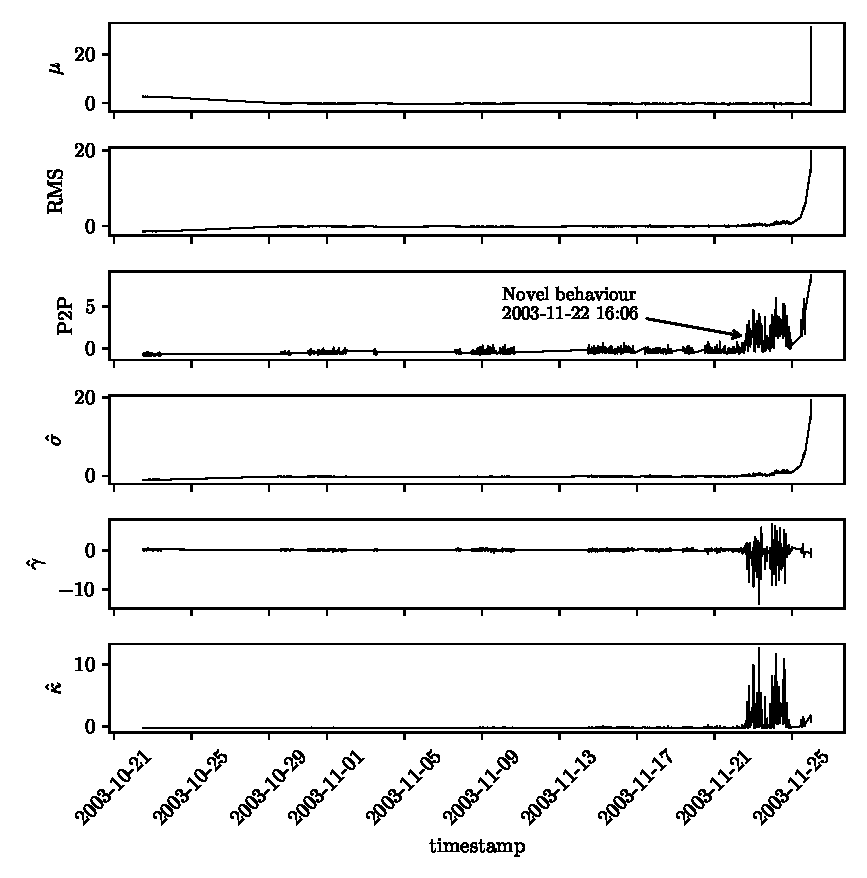
\includegraphics[scale=1]{images/FeatureExtraction/TDfeatures.pdf}
    \caption{All time-domain features for the \quoted{Bearing 3 x} vibration signal from the \gls{ims} dataset}
    \label{fig:IMS_TD_features}
\end{figure}

To visualise the evolution of the features over time, let's consider the all the snapshots of the \quoted{Bearing 3 x} signal from the \gls{ims} dataset and plot all the time-domain features described above. The result is shown in \autoref{fig:IMS_TD_features}. Having seen also \autoref{fig:IMS_bearing}, it's not surprising that the P2P and the kurtosis are the time domain features that capture the degradation of the bearing the earliest. 


\section{Frequency-domain features}

To capure also the frequency behaviour of the signal, other tools are needed. In this section, we will describe the frequency-domain features  $\vect{F}_f = \{F_{m+1}, F_{m+2}, \dots, F_l\}$ that will be used in the developed framework.

\subsection{Fourier transform}

One powerful tool to analyse the frequency content of a signal is the fourier transform or, in the case of a discrete signal, the Discrete Fourier Transform(\gls{dft}), that has a very efficient implementation in the Fast Fourier Transform (\gls{fft}) algorithm \cite{cooley1965algorithm}. This algorithm is implemented in many programming languages and libraries, including \texttt{python} and \texttt{C}. The theory behing this topic is breafly described in \autoref{app:FFT}. 

To have a better understanding of the capability of the \gls{fft} to capture the frequency content of a signal (and the presence of a disturbance in a partion of the signal), let's consider the following signal, composed by the sum of four sinusoids with different frequencies that is plotted with its \gls{dft} in \autoref{fig:FD_known}:
\begin{multline}
    x(t) = \sin(2\pi f_1 t) + \sin(2\pi f_2 t) + \sin(2\pi f_3 t) + \sin(2\pi f_4 t), \\
    t \in [0, 1], \quad \{f_1, f_2, f_3, f_4\} = \{2, 5, 7, 15\} \si{\Hz}
\end{multline}

In the \autoref{fig:FD_known} it is possible to see the four peaks in the frequency domain, corresponding to the four frequencies of the sinusoids. Now, let's consider the same signal, but with an additive disturbance in a small portion of the signal, as shown in \autoref{fig:FD_known_dist}. The disturbance is a period of the signal $x(t) = \sin(2\pi f_5 t)$, with $f_5=50\si{\Hz}$, that is added to the signal in the interval $t \in [0.4, 0.6]$. The \gls{dft} of this signal is shown in \autoref{fig:FD_known_dist}. It is possible to see that the disturbance is captured by the spectrum, but as a broad frequency additional components, insteas ofa peack at $f_5=50\si{\Hz}$. This is because the disturbance is not acting on the whole signal. For our purpose, this is still good because we can detect the variation of all the frequencies involved.

Consider the period of the undisturbed signal, that is the \gls{lcm} of the periods of the four sinusoids composing the signal.
\[ 
    T = \text{LCM} \left( \frac{1}{2} \si{\s},\frac{1}{5}\si{\s},\frac{1}{7}\si{\s},\frac{1}{15}\si{\s} \right) = 1 \si{\s}
\]

So, we were looking to a signal that has a signal of one second, sampled for exactly one second. Let's see what happens if we sample the same signal for a time that is not an integer multiple of the period. In \autoref{fig:FD_known_leackage} it is shown the \gls{dft} of the same signal as before, but sampled for $t \in [0, 0.9]$. It is possible to see that the peaks are still at the frequencies of the sinusoids composing the signal, but they are not single points as it appears that also frequencies near the true frequencies are present. This phenomenon is called \emph{spectral leackage} and happens because the signal is not sampled for an integer number of periods \cite{SpectralLeakage}. 


\begin{figure}
    \centering
    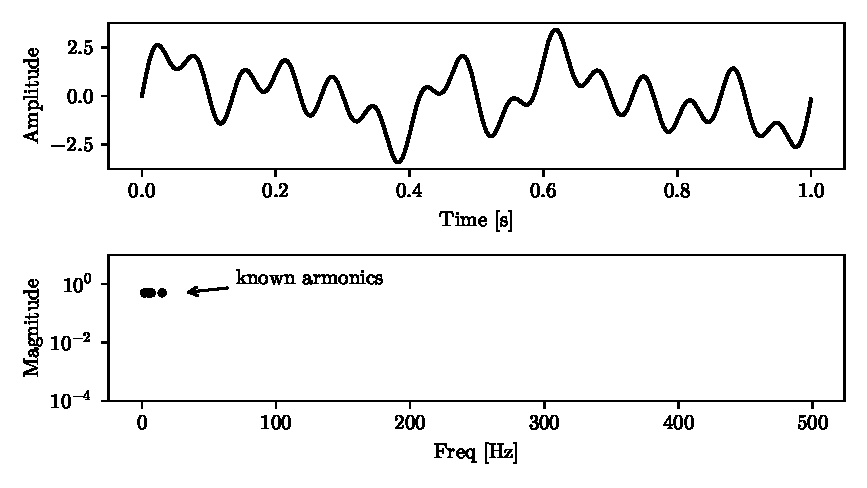
\includegraphics[scale=1]{images/FeatureExtraction/FD_known.pdf}
    \caption{FFT of the signal with known frequency components}
    \label{fig:FD_known}
\end{figure}

\begin{figure}
    \centering
    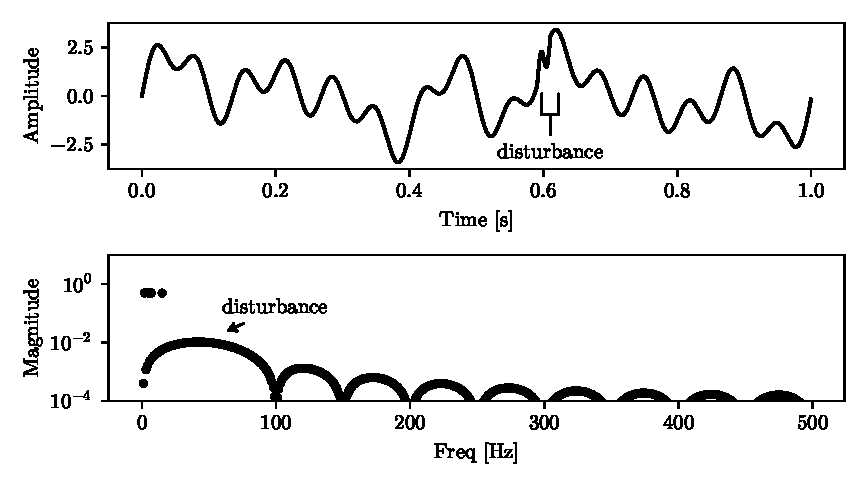
\includegraphics[scale=1]{images/FeatureExtraction/FD_known_dist.pdf}
    \caption{FFT of the signal with known frequency components, and an additive disturbance}
    \label{fig:FD_known_dist}
\end{figure}

\begin{figure}
    \centering
    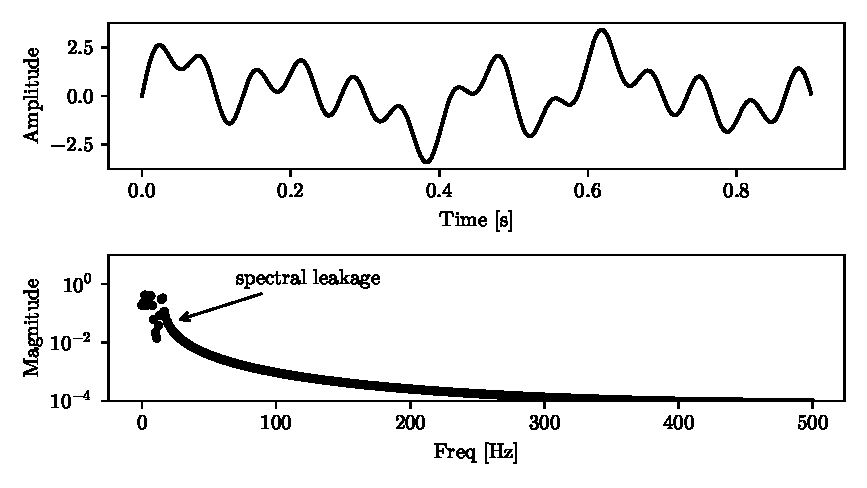
\includegraphics[scale=1]{images/FeatureExtraction/FD_known_outofsync.pdf}
    \caption{FFT of the signal with known frequency components, with a domain that is not an integer multiple of the period}
    \label{fig:FD_known_leackage}
\end{figure}

\begin{figure}
    \centering
    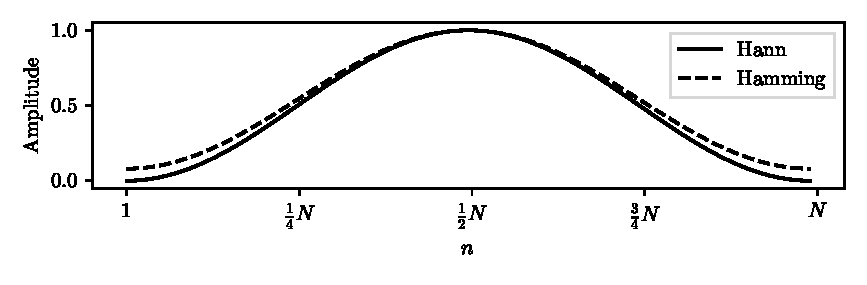
\includegraphics[scale=1]{images/FeatureExtraction/windows.pdf}
    \caption{Hann and Hamming windows}
    \label{fig:windows}
\end{figure}


\subsection{Preprocessing}
Up to now, it has been shown that the \gls{dft} will translate the presence of a disturbance in the time domain into several periodic components in the frequency domain. But it has the weakness of the spectral leackage if the sampling interval is not an integer multiple of the period of the signal that is the most likely scenario in a real application. To compensate this fenomena, it is better to use a trasformation to the signal that make it artificially stant and end with the same value. This can be done with a \emph{windowing} function, or with the \quoted{flip and reverse} method \cite{Preprocessing}. 

The most common windowing funcitons are the \emph{Hann} and the \emph{Hamming} windows, defined as:
\begin{eqnarray}
    w_{hann}(n) = 0.5\; \left[1 - \cos \left ( \frac{2 \pi n}{N} \right) \right] \\
    w_{hamming}(n) = \frac{25}{46}\; \left[1 - \cos \left ( \frac{2 \pi n}{N} \right) \right]
\end{eqnarray}
where $N$ is the total number of samples. Those funcitons are plotted in \autoref{fig:windows}. The preprocessing operation is simply to multiply the signal by the windowing function. this will make the first and last point of the signal exactly zero in the case of the Hann window, and very close to zero in the case of the Hamming window but with the advantage of having a narrower peak in the spectrum. The \quoted{flip and reverse} method is simply to subtract a flipped and reversed copy of the signal to itself, i.e. $x_{new}(n) = x(n) - x(N-n) \, \forall n \in [1,N]$. A comparison of those preprocessing techniques is shown in \autoref{fig:FD_preprocessing} and \autoref{fig:FD_preprocessing_dist}. In both figures, it is evident that the \quoted{flip and reverse} method generate a fake peak at half the sampling frequency, while the windowing funciton don't. Moreover, looking at \autoref{fig:FD_preprocessing_dist}, it is possible to see that the Hann window better suppress the spectral leackage.
In figure \autoref{fig:IMS}, it is shown the effect of different preprocessing techniques on a real world signal from the \gls{ims} dataset. The Hann window will be implicitly used in the the rest of this section.



\begin{figure}
    \centering
    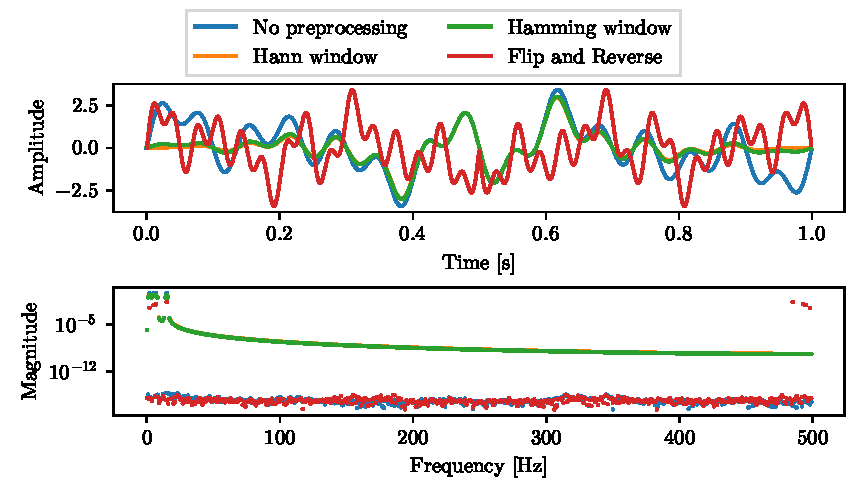
\includegraphics[scale=1]{images/FeatureExtraction/FD_Preproc_sync.pdf}
    \caption{FFT of the signal  with a domain that is an integer multiple of the period, and a preprocessing technique applied}
    \label{fig:FD_preprocessing}
\end{figure}

\begin{figure}
    \centering
    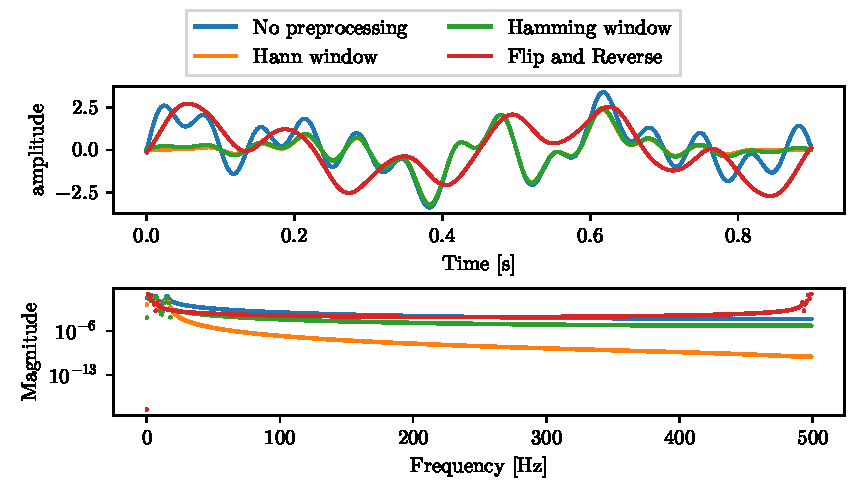
\includegraphics[scale=1]{images/FeatureExtraction/FD_Preproc_outofsync.pdf}
    \caption{FFT of the signal with a domain that is not an integer multiple of the period, and a preprocessing technique applied,}
    \label{fig:FD_preprocessing_dist}
\end{figure}

\begin{figure}
    \centering
    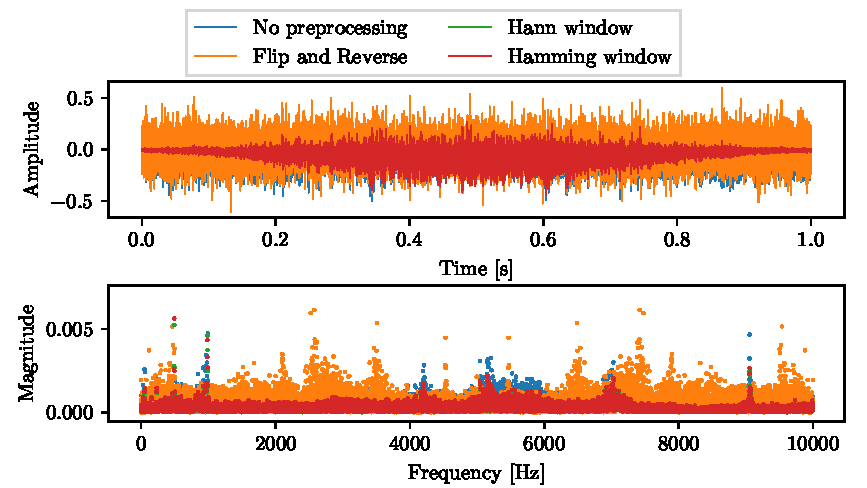
\includegraphics[scale=1]{images/FeatureExtraction/FD_PreprocIMS.pdf}
    \caption{FFT of the \quoted{Bearing 3 x} vibration signal from the \gls{ims} dataset, in normal conditions and with preprocessing techniques applied}
    \label{fig:IMS}
\end{figure}

\section{Conclusions}
Even just considering very simple time-domain features, we can already detect the degradation of the bearing comparing this features values to a threshold. On the other hand, also the frequency-domain features could be just compared with a threshold to detect the novel behaviours. But, as we will see in \autoref{ch:Framework}, a general purpose framework based upon a more sophisticated approach based on the clustering of the data, it will be possible to condense all the features from all the signals into a single metric that will be used to detect the novel behaviour. This will have several advantages. Some ot them are being able to detect a novel behaviour even if it is not possible to define a threshold for each feature, and the single threshold to be defined on the metric will be easier to interpret and tune. Moreover, the framework will be able to detect the novelty even earlier and even if the degradation of the bearing is not captured by the time-domain features, but only by the frequency-domain features.

